\documentclass[a4paper, 12pt]{article}

\usepackage[english,russian]{babel}
\usepackage[T2A]{fontenc}
\usepackage[utf8]{inputenc}
\usepackage{geometry}
\usepackage{enumitem}
\usepackage{setspace}
\usepackage{amssymb}
\usepackage{graphicx}
\usepackage{wrapfig}
\usepackage{float}
\usepackage{amsmath}
\usepackage{textcomp}
\usepackage{dsfont}

\geometry{top=5mm, left=1cm}
%\setlength{\parindent}{0}
\renewcommand{\arraystretch}{1.2}
\linespread{1}

\begin{document}
    \begin{center}
        \textbf{Сферическая геометрия №2}\\
        Сечения сферы
    \end{center}

    \textbf{№1} Расстояние от центра сферы радиуса R до секущей плоскости равно $d$.
    Вычислите радиус окружности, полученной в сечении плоскостью.

    \textbf{Решение}\\

    \begin{center}
        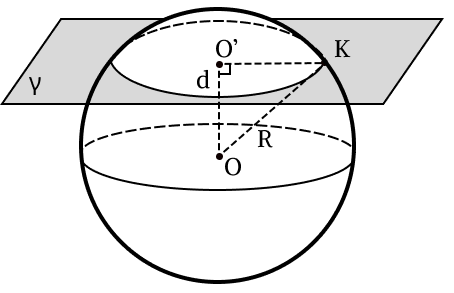
\includegraphics[width=0.2\textwidth]{images/img1}\\
    \end{center}

    \[  O'K =  \sqrt{R ^ 2 - d ^ 2} \]


    Ответ: $r = \sqrt{R ^ 2 - d ^ 2}$\\


    \textbf{№2} Секущая плоскость проходит через конец диаметра сферы радиуса $R$ так,
    что угол между диаметром и плоскостью равен $\alpha$.
    Найдите длину окружности, получившейся в сечении.

    \textbf{Решение}\\

    \begin{center}
        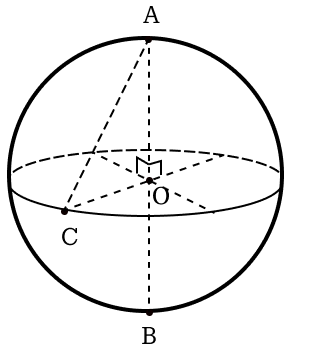
\includegraphics[width=0.2\textwidth]{images/img2}\\
    \end{center}

    \[\angle Q'KO = \alpha , OK = R\]
    \[ r = R * \cos \alpha \]
    \[ L = 2\pi r = 2 \pi R  \cos \alpha \]

    Ответ: $L = 2\pi r = 2 \pi R  \cos \alpha$\\


    \textbf{№3}
    Покажите, что если плоскость проходит через центр сферы, то она содержит ее диаметр.

    \textbf{Решение}\\

    Если плоскость проходит через центр сферы, то расстояние от центра сферы до плоскости равно нулю.
    Тогда радиус полученной в сечении окружности равен радиусу сферы, а значит любой диаметр окружности является диаметром сферы.\\


    \textbf{№4}
    Покажите, что сферической прямой соответствует единственная пара полюсов.

    \textbf{Решение}\\

    Предположим, что существует две пары полюсов, тогда из центра сферы восстановлены два перпендикуляра к плоскости сечения,
    что противоречит теореме о единственности перпендикуляра, проведенного из точки к плоскости.\\

    Таким образом, существует не более 1 пары полюсов, соответствующих прямой на сфере.\\

    Существование следует из той же теоремы о прямой, перпендикулярной к плоскости.\\


    \textbf{№5}
    Покажите, что двум диаметрально противоположным точкам на сфере соответствует единственная поляра.

    \textbf{Решение}\\

    Предположим, что это не так, тогда через центр проходит две плоскости, перпендикулярные к диаметру, проходящему через полюсы.
    Тогда такие плоскости параллельны по теореме о плоскостях перпендикулярных к одной прямой,
    а так как они имеют общую точку центр сферы, то они совпадают.\\


    \textbf{№6}
    Покажите, что cуществует единственная сферическая прямая, проходящая через две данные различные точки,
    кроме случая, когда эти точки диаметрально противоположны;
    тогда таких прямых бесконечно много.

    \textbf{Решение}\\

    1) Точки не диаметрально противоположные.
    В этом случае можно воспользоваться аксиомой стереометрии и рассмотреть три точки: два полюса и центр сферы.
    Тогда эти точки не лежат на одной прямой, а значит задают единственную плоскость.
    Любая плоскость, содержащая центр сферы будет высекать большую окружность(и наоборот), то есть являться прямой на сфере,
    единственность следует из замечания выше.

    2) Если точки диаметрально противоположные, то они лежат на диаметре, то есть центр сферы и полюсы лежат на одной прямой,
    тогда через эту прямую можно провести бесконечное количество плоскостей, которые будут содержать диаметр, а значит
    высекать большую окружность, что соответствует определению прямой на сфере.\\


    \textbf{№7}
    Постройте параллельные сферические прямые или докажите, что это невозможно.

    \textbf{Решение}\\

    Сферические прямые являются диаметральными сечениями сферы, а значит их
    плоскости пересекаются по диаметру, то есть прямые имеют две общие диаметрально
    противоположные точки.

    Таким образом, любые две сферические прямые пересекаются, а значит параллельных прямых на сфере не существует.\\


    \textbf{№8}
    Точки $A$ и $C$ - полярно сопряженные на окружности радиуса $R$.
    Найдите евклидово расстояние между этими точками.

    \textbf{Решение}\\

    \begin{center}
        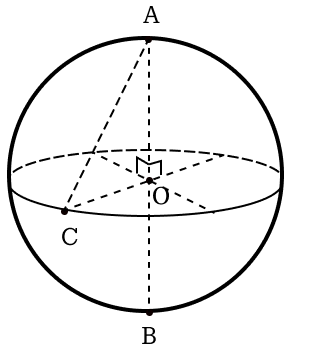
\includegraphics[width=0.2\textwidth]{images/img2}\\
    \end{center}

    Для определенности будем считать, что точка $A$ - полюс, а точка $C$ лежит на поляре полюса.\\

    Так как поляра является большой окружностью, то ее радиус равен радиусу сферы, а так как $AB$ - перпендикуляр,
    то по теореме Пифагора получаем:
    \[
        AC = \sqrt {CO ^ 2 + AO ^ 2} = \sqrt {R ^ 2 + R ^ 2} = R\sqrt {2}
    \]

    Ответ: $R\sqrt{2}$\\


    \textbf{№9}
    Когда поляры(плоскости) трех точек пересекаются по прямой?

    \textbf{Решение}\\

    1) Рассмотрим случай, когда три точки лежат на одной прямой.

    \begin{center}
        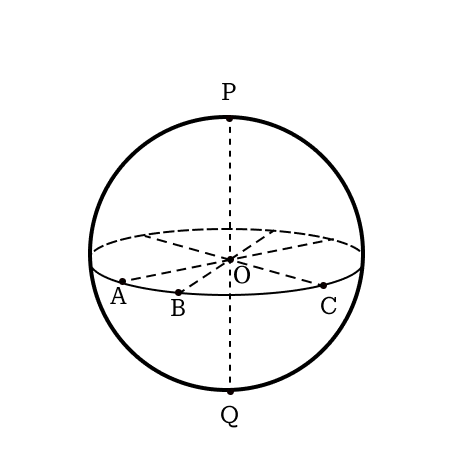
\includegraphics[width=0.2\textwidth]{images/Frame 70}\\
    \end{center}

    Тогда PQ - является перпендикулярным к прямой, содержащей точки диаметром,
    а так как плоскость поляры точки есть множество перпендикулярных прямых,
    проведенных через центр сферы к диаметру, проведенному через точку, то она содержит PQ, а так как PQ
    перпендикулярна плоскости прямой, содержащей точки, то она перпендикулярна
    всякой прямой, проведенной в этой плоскости, в частности она перпендикулярна всем диаметрам,
    проведенным через данные точки, то есть лежит в плоскости поляры каждой точки, а
    значит является пересечением поляр.

    2) Рассмотрим случай, когда три точки не лежат на одной прямой.\\

    Допустим, что PQ - соединяет полюсы поляры, проведенной через точки AB, а
    ED - соединяет полюсы поляры, проведенной через точки BC.\\

    Допустим, что эти отрезки совпадают, ведь иначе пересечение поляр трех точек есть центр сферы.
    Тогда получается, что PQ перпендикулярен плоскости AB и PQ перпендикулярен плоскости BC,
    а значит эти плоскости параллельны, но а так как они имеют общую точку B, то они совпадают,
    но тогда получается, что прямая AB совпадает с прямой BC, то есть A, B, C лежат на одной прямой - противоречие.

    Ответ: когда три точки лежат на одной прямой.
    \begin{center}
        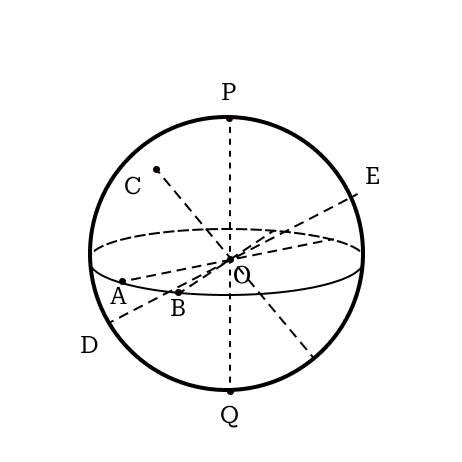
\includegraphics[width=0.2\textwidth]{images/Frame 71}\\
    \end{center}\\


    \textbf{№10}
    При каком условии две прямые на сфере содержат полюсы друг друга?

    \textbf{Решение}\\

    Так как плоскости содержат полюсы друг друга, то они содержат перпендикуляры друг друга,
    что по признаку перпендикулярности плоскостей означает перпендикулярность плоскостей.

    Ответ: при условии перпендикулярности плоскостей, задающих прямые на сфере.\\


    \textbf{№11}
    Чему равна площадь евклидового треугольника, образованного двумя полисами и полярно сопряженной с ними точкой,
    если радиус сферы $R$.

    \textbf{Решение}\\

    \begin{center}
        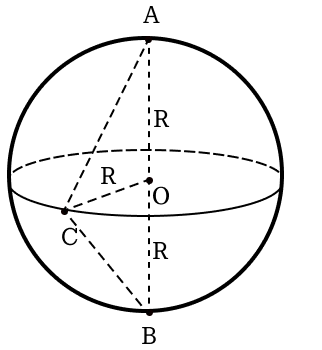
\includegraphics[width=0.2\textwidth]{images/img6}\\
    \end{center}

    1) $AB \bot CO$ по определению полюсов.\\

    2)\[
          S_{\triangle ABC} = \frac{1}{2} CO * AB = \frac{1}{2} R * 2R = R ^ 2
    \]

    Ответ: $R ^ 2$\\





\end{document}
